%% Copernicus Publications Manuscript Preparation Template for LaTeX Submissions
%DIF LATEXDIFF DIFFERENCE FILE
%DIF DEL original.tex   Tue Dec 20 20:11:45 2016
%DIF ADD revision.tex   Tue Dec 20 20:08:33 2016
%% ---------------------------------
%% This template should be used for copernicus.cls
%% The class file and some style files are bundled in the Copernicus Latex Package which can be downloaded from the different journal webpages.
%% For further assistance please contact the Copernicus Publications at: publications@copernicus.org
%% http://publications.copernicus.org


%% Please use the following documentclass and Journal Abbreviations for Discussion Papers and Final Revised Papers.


%% 2-Column Papers and Discussion Papers
\documentclass[journal abbreviation, manuscript]{copernicus}



%% Journal Abbreviations (Please use the same for Discussion Papers and Final Revised Papers)

% Archives Animal Breeding (aab)
% Atmospheric Chemistry and Physics (acp)
% Advances in Geosciences (adgeo)
% Advances in Statistical Climatology, Meteorology and Oceanography (ascmo)
% Annales Geophysicae (angeo)
% ASTRA Proceedings (ap)
% Atmospheric Measurement Techniques (amt)
% Advances in Radio Science (ars)
% Advances in Science and Research (asr)
% Biogeosciences (bg)
% Climate of the Past (cp)
% Drinking Water Engineering and Science (dwes)
% Earth System Dynamics (esd)
% Earth Surface Dynamics (esurf)
% Earth System Science Data (essd)
% Fossil Record (fr)
% Geographica Helvetica (gh)
% Geoscientific Instrumentation, Methods and Data Systems (gi)
% Geoscientific Model Development (gmd)
% Geothermal Energy Science (gtes)
% Hydrology and Earth System Sciences (hess)
% History of Geo- and Space Sciences (hgss)
% Journal of Sensors and Sensor Systems (jsss)
% Mechanical Sciences (ms)
% Natural Hazards and Earth System Sciences (nhess)
% Nonlinear Processes in Geophysics (npg)
% Ocean Science (os)
% Proceedings of the International Association of Hydrological Sciences (piahs)
% Primate Biology (pb)
% Scientific Drilling (sd)
% SOIL (soil)
% Solid Earth (se)
% The Cryosphere (tc)
% Web Ecology (we)
% Wind Energy Science (wes)


%% \usepackage commands included in the copernicus.cls:
%\usepackage[german, english]{babel}
%\usepackage{tabularx}
%\usepackage{cancel}
%\usepackage{multirow}
%\usepackage{supertabular}
%\usepackage{algorithmic}
%\usepackage{algorithm}
%\usepackage{amsthm}
%\usepackage{float}
%\usepackage{subfig}
%\usepackage{rotating}
\usepackage{color,soul}
%DIF < 
%DIF PREAMBLE EXTENSION ADDED BY LATEXDIFF
%DIF UNDERLINE PREAMBLE %DIF PREAMBLE
\RequirePackage[normalem]{ulem} %DIF PREAMBLE
\RequirePackage{color}\definecolor{RED}{rgb}{1,0,0}\definecolor{BLUE}{rgb}{0,0,1} %DIF PREAMBLE
\providecommand{\DIFadd}[1]{{\protect\color{blue}\uwave{#1}}} %DIF PREAMBLE
\providecommand{\DIFdel}[1]{{\protect\color{red}\sout{#1}}}                      %DIF PREAMBLE
%DIF SAFE PREAMBLE %DIF PREAMBLE
\providecommand{\DIFaddbegin}{} %DIF PREAMBLE
\providecommand{\DIFaddend}{} %DIF PREAMBLE
\providecommand{\DIFdelbegin}{} %DIF PREAMBLE
\providecommand{\DIFdelend}{} %DIF PREAMBLE
%DIF FLOATSAFE PREAMBLE %DIF PREAMBLE
\providecommand{\DIFaddFL}[1]{\DIFadd{#1}} %DIF PREAMBLE
\providecommand{\DIFdelFL}[1]{\DIFdel{#1}} %DIF PREAMBLE
\providecommand{\DIFaddbeginFL}{} %DIF PREAMBLE
\providecommand{\DIFaddendFL}{} %DIF PREAMBLE
\providecommand{\DIFdelbeginFL}{} %DIF PREAMBLE
\providecommand{\DIFdelendFL}{} %DIF PREAMBLE
%DIF END PREAMBLE EXTENSION ADDED BY LATEXDIFF

\begin{document}

\title{Enabling BOINC in \DIFdelbegin \DIFdel{Cloud Services: Climateprediction.net }\DIFdelend \DIFaddbegin \DIFadd{Infrastructure }\DIFaddend as \DIFdelbegin \DIFdel{Example}\DIFdelend \DIFaddbegin \DIFadd{a Service Cloud Systems}\DIFaddend }

% \Author[affil]{given_name}{surname}
\Author[1]{Diego}{Montes}
\Author[1,2]{Juan A.}{A\~nel}
\Author[3]{Tom\'as}{F. Pena}
\DIFdelbegin %DIFDELCMD < \Author[4]{David}{C. H. Wallom}
%DIFDELCMD < %%%
\DIFdelend \DIFaddbegin \Author[4,5]{Peter}{Uhe}
\Author[5]{David}{C. H. Wallom}
\DIFaddend %\Author[]{}{}
%\Author[]{}{}
%\Author[]{}{}

\DIFdelbegin %DIFDELCMD < \affil[1]{Facultade de Ciencias, Universidade de Vigo, Ourense, 32004, Spain}
%DIFDELCMD < %%%
\DIFdelend \DIFaddbegin \affil[1]{EPhysLab, Universidade de Vigo, Ourense, 32004, Spain}
\DIFaddend \affil[2]{Smith School of Enterprise and the Environment, University of Oxford, Oxford, UK}
\DIFdelbegin %DIFDELCMD < \affil[3]{ Centro de Investigaci\'on en Tecnolox\'ias da Informaci\'on (CITIUS), University of Santiago de Compostela, Santiago de Compostela, 15782, Spain}
%DIFDELCMD < \affil[4]{Oxford e-Research Centre, University of Oxford, OX1 3QG, UK.}
%DIFDELCMD < 
%%%
\DIFdelend \DIFaddbegin \affil[3]{Centro de Investigaci\'on en Tecnolox\'ias da Informaci\'on (CITIUS), University of Santiago de Compostela, Santiago de Compostela, 15782, Spain}
\affil[4]{School of Geography and the Environment, University of Oxford, Oxford, UK}
\affil[5]{Oxford e-Research Centre, University of Oxford, OX1 3QG, UK.}
\DIFaddend 

%% The [] brackets identify the author with the corresponding affiliation. 1, 2, 3, etc. should be inserted.

\runningtitle{Enabling BOINC in Cloud Services}

\runningauthor{Diego Montes}

\correspondence{Diego Montes (kabute@uvigo.es)}



\received{}
\pubdiscuss{} %% only important for two-stage journals
\revised{}
\accepted{}
\published{}

%% These dates will be inserted by Copernicus Publications during the typesetting process.


\firstpage{1}

\maketitle



\begin{abstract}
Volunteer \DIFdelbegin \DIFdel{computing is increasingly being used }\DIFdelend \DIFaddbegin \DIFadd{or Crowd computing is becoming increasingly popular }\DIFaddend to solve complex \DIFdelbegin \DIFdel{problems, in an increasing number of projects from all manner of different research areas. Several }\DIFdelend \DIFaddbegin \DIFadd{research problems, from an increasing diverse range of areas. The majority }\DIFaddend of these have been built \DIFdelbegin \DIFdel{on }\DIFdelend \DIFaddbegin \DIFadd{using }\DIFaddend the Berkeley Open Infrastructure for Network Computing (BOINC) platform, which provides a range of different services to manage \DIFdelbegin \DIFdel{any project. Nowadays BOINC is widely used in scientific research to foster low-cost distributed infrastructure using volunteers' computers. Among the better known projects launched using BOINC are climateprediction.
net, SETI@Home or LHC@Home.

}\DIFdelend \DIFaddbegin \DIFadd{all computation aspects of a project. The BOINC system is ideal in those cases where not only does the research community involved need low cost access to massive computing resource but also that there is a significant public interest in the research done.
}\DIFaddend 

We discuss the \DIFdelbegin \DIFdel{ways }\DIFdelend \DIFaddbegin \DIFadd{way }\DIFaddend in which Cloud services can help BOINC based projects to deliver results \DIFdelbegin \DIFdel{faster in responsive mode; this }\DIFdelend \DIFaddbegin \DIFadd{in a fast, on demand manner. This }\DIFaddend is difficult to achieve using volunteers\DIFdelbegin \DIFdel{but }\DIFdelend \DIFaddbegin \DIFadd{, and }\DIFaddend at the same time\DIFdelbegin \DIFdel{it optimizes }\DIFdelend \DIFaddbegin \DIFadd{, using scalable cloud resources for short on demand projects can optimize }\DIFaddend the use of the available resources. We show how this design can be used as an efficient distributed computing platform within the Cloud, and outline new approaches that could open up new possibilities in this field, using \DIFdelbegin \DIFdel{climateprediction}\DIFdelend \DIFaddbegin \DIFadd{climate}\textit{\DIFadd{prediction}}\DIFaddend .net as a case study.

\keywords{BOINC, Cloud, CPDN, Volunteer computing}
\end{abstract}

\introduction
{T}{raditionally}, climate models have been run using supercomputers because of their vast computational \DIFdelbegin \DIFdel{needs }\DIFdelend \DIFaddbegin \DIFadd{complexity }\DIFaddend and high cost. Since its early development\DIFaddbegin \DIFadd{, }\DIFaddend climate modelling has been an undertaking that has tested the limits of High-Performance Computing (HPC). \DIFdelbegin \DIFdel{It has more recently become a task better described as High-Throughput computing (HTC), becausefor some simulations }\DIFdelend \DIFaddbegin \DIFadd{This application of models to answer different types of questions has led to them being used in manners not originally foreseen. This is because, for some types of  simulations, }\DIFaddend it can take several months to finish a modelling experiment given the \DIFdelbegin \DIFdel{vast computational }\DIFdelend \DIFaddbegin \DIFadd{scale of }\DIFaddend resources involved. One reason for including climate modelling as \DIFdelbegin \DIFdel{an HTC}\DIFdelend \DIFaddbegin \DIFadd{a High-Throughput Computing (HTC), }\DIFaddend as opposed to an HPC problem is due to the \DIFdelbegin \DIFdel{generally high number of small }\DIFdelend \DIFaddbegin \DIFadd{application design model, where there is a number }\DIFaddend (not usually greater than twenty) \DIFaddbegin \DIFadd{of }\DIFaddend uncoupled, long-running tasks, each corresponding to a single climate simulation and its results.

The aim of increasing the total number of members in an ensemble of climate simulations, together with the need to achieve increased computational power to better represent the physical and chemical processes being modelled, has been well understood for some decades in meteorological and climate research. Climate models make use of ensemble means to improve the accuracy of the results and \DIFdelbegin \DIFdel{minimize errors}\DIFdelend \DIFaddbegin \DIFadd{quantify uncertainty}\DIFaddend , but the number of members in each ensemble tends to be small due to computational constraints. The overwhelming majority of research projects use ensembles that generally contain only a very small number of simulations, which has an obvious impact in terms of the statistical uncertainty of the results.


The \DIFdelbegin \DIFdel{ClimatePrediction}\DIFdelend \DIFaddbegin \DIFadd{climate}\textit{\DIFadd{prediction}}\DIFaddend .net project (\DIFdelbegin \DIFdel{also known as }\DIFdelend CPDN) was created in 1999\DIFaddbegin \DIFadd{~}\DIFaddend \citep{allen1999,CPDNweb} as a distributed computing initiative to address the uncertainties described above. \DIFdelbegin \DIFdel{The aim of CPDN }\DIFdelend \DIFaddbegin \DIFadd{Its aim }\DIFaddend is to run thousands of different climate modelling simulations in order to research the uncertainties associated with some of the parameters\DIFdelbegin \DIFdel{, which }\DIFdelend \DIFaddbegin \DIFadd{. This }\DIFaddend is essential for understanding how small changes or variations in initial conditions can affect both the models themselves and the results of climate simulations. The project is currently run by the University of Oxford using volunteer computing via the BOINC (Berkeley Open Infrastructure for Network Computing) framework\DIFaddbegin \DIFadd{~}\DIFaddend \citep{boinc:Online, anderson2004}. In its early use of distributed computing, CPDN became a precursor of the Many-Task Computing (MTC) paradigm\DIFaddbegin \DIFadd{~}\DIFaddend \citep{raicu2008}.

\DIFdelbegin \DIFdel{Today }\DIFdelend CPDN has been running for more than 10 years and \DIFdelbegin \DIFdel{is currently facing a different set of }\DIFdelend \DIFaddbegin \DIFadd{faces a number of evolving }\DIFaddend challenges:
\begin{itemize}

\item \DIFdelbegin \DIFdel{a growing }\DIFdelend \DIFaddbegin \DIFadd{an  increasing }\DIFaddend and variable need for new \DIFdelbegin \DIFdel{resources, thanks to the release of, and outputs from, new versions of the model together with the processing of huge amounts of data that are difficult to manage using the current infrastructure within the BOINC framework;
}\DIFdelend \DIFaddbegin \DIFadd{computational and storage resources;
}\item \DIFadd{the processing power and memory of current volunteers' computers, restricts the use of more complex models and higher resolution.
}\DIFaddend \item \DIFdelbegin \DIFdel{a lack of , and a need for, greater control over the workflow and its intermediate stages;
}%DIFDELCMD < \item %%%
\item%DIFAUXCMD
\DIFdelend the need to \DIFdelbegin \DIFdel{streamline }\DIFdelend \DIFaddbegin \DIFadd{manage }\DIFaddend costs and budgeting. This is of particular interest in researching on-demand projects \DIFdelbegin \DIFdel{increasingly being }\DIFdelend requested by external research collaborators and stakeholders;
\end{itemize}

To address these issues we have explored the combination of MTC\DIFaddbegin \DIFadd{/volunteer }\DIFaddend and Cloud computing as a possible improvement \DIFdelbegin \DIFdel{on, and alternative }\DIFdelend \DIFaddbegin \DIFadd{or, extension }\DIFaddend to, a real existing project. This kind of solution has previously been proposed for scientific purposes by\DIFdelbegin \DIFdel{Iosup et al. }\DIFdelend \DIFaddbegin \DIFadd{~\mbox{%DIFAUXCMD
\cite{iosup2011} }%DIFAUXCMD
}\DIFaddend and is supported by initiatives such as Microsoft Azure for Research\DIFdelbegin \DIFdel{\mbox{%DIFAUXCMD
\citep{azure2014}}%DIFAUXCMD
. Here we describe an initial assessment of the current state of the project and propose the implementation of the following }\DIFdelend \DIFaddbegin \DIFadd{~\mbox{%DIFAUXCMD
\citep{azure2014}}%DIFAUXCMD
.
}\section{\DIFadd{Background}}
\DIFadd{It is not the aim of this paper to describe the internals of BOINC, and for better comprehension of the problem that we are trying to solve,  it is recommended to review previous works about this knowledge such as~\mbox{%DIFAUXCMD
\cite{Ries2011}}%DIFAUXCMD
.
}

\subsection{\DIFadd{Problem Description}}

\DIFadd{Here we describe  some of the problems that we intend to address, as well as proposed implementations of possible }\DIFaddend solutions:

\begin{itemize}

\item \DIFaddbegin \DIFadd{to run more complex and computationally more expensive versions of the model, resources greater than volunteer computers can provide may be needed. One solution is }\DIFaddend a re-engineering and deployment of the client side from a volunteer computing architecture to an Infrastructure as a Service (IaaS) based on Cloud Computing (\DIFdelbegin \DIFdel{over }\DIFdelend \DIFaddbegin \DIFadd{e.g. }\DIFaddend Amazon Web Services, AWS)\DIFdelbegin \DIFdel{. This new infrastructure will handle both the computing, based on AWS EC2 (Elastic Compute Cloud, Amazon's solution for Cloud Computing) instances, and (shared) storage needs using S3 buckets (Simple Storage Service, Amazon's Simple Cloud Storage);
}%DIFDELCMD < \item %%%
\item%DIFAUXCMD
\DIFdel{design and development of a Control Plane using a system composed of a RESTful backend (an Application Programming Interface (API) coded in Python (using Flask, a web microframework)), using Boto to communicate with the AWS API, and SQLite3 (as a local status Database) to control the execution of the simulations, together with a frontend to display the statistics (using HTML5 and the JQuery/jqPlot libraries), information and metrics;
}%DIFDELCMD < \item %%%
\item%DIFAUXCMD
\DIFdel{complete documentation of the process, allowing knowledge to be transferred or migrated easily to other systems;
}%DIFDELCMD < \end{itemize}
%DIFDELCMD < 
%%%
\DIFdelend \DIFaddbegin \DIFadd{;
}\DIFaddend 

\DIFdelbegin \DIFdel{Furthermore, in this work we wish to prove the feasibility of running a state-of-the-art climate model in a Cloud environment. Although no problem has yet been conceived that would benefit from such an approach, to the best of our knowledge, this has never previously been attempted.

}%DIFDELCMD < 

%DIFDELCMD < %%%
\DIFdel{The remainder of this paper is organized as follows. We begin with a section explaining the background to the problem and the essential elements of BOINC. We then include a section explaining the solution being tested, and finally, the results are discussed in the conclusion.

}%DIFDELCMD < 

%DIFDELCMD < 
%DIFDELCMD < %%%
\section{\DIFdel{Background}}

%DIFAUXCMD
\addtocounter{section}{-1}%DIFAUXCMD
%DIFDELCMD < 

%DIFDELCMD < %%%
\DIFdel{Although it is not our aim to describe the full migration of the BOINC server side (only the Data Server), and our interest lies in the client side of the current infrastructure (where all the computational load applies), it seems necessary to include a high-level technical description, in order to clarify the problem we are trying to solve.

}%DIFDELCMD < 

%DIFDELCMD < %%%
\DIFdel{In the Figure~\ref{fig:boinchla}, we show the high-level architecture of BOINC. The server section contains a number of different elements:

}%DIFDELCMD < 

%DIFDELCMD < \begin{itemize}
%DIFDELCMD <  %%%
\DIFdelend \item \DIFdelbegin \DIFdel{task server: scheduling and dispatching jobs to clients;
 }%DIFDELCMD < \item %%%
\item%DIFAUXCMD
\DIFdel{data server:  sending and receiving workunits to/from BOINC clients;
 }%DIFDELCMD < \item %%%
\item%DIFAUXCMD
\DIFdel{databases and storage: there are 2 Databases, one for BOINC itself and another for the project-defined application. There is also a system for File storage used by the Data Server;
}%DIFDELCMD < \end{itemize}
%DIFDELCMD < %%%
%DIF < 
\DIFdel{At a lower level up to 5 daemons are used for the Task and Data servers:
 }%DIFDELCMD < \begin{itemize}
\begin{itemize}%DIFAUXCMD
%DIFDELCMD <  \item %%%
\item%DIFAUXCMD
\DIFdel{scheduler: decides how jobs are dispatched to clients;
 }%DIFDELCMD < \item %%%
\item%DIFAUXCMD
\DIFdel{feeder: communicates database information to the scheduler CGI (Common Gateway Interface) via shared memory;
 }%DIFDELCMD < \item %%%
\item%DIFAUXCMD
\DIFdel{transitioner: controls the changes of state for the results;
 }%DIFDELCMD < \item %%%
\item%DIFAUXCMD
\DIFdel{validator: validates that the sent result is valid;
 }%DIFDELCMD < \item %%%
\item%DIFAUXCMD
\DIFdel{assimilator: used to assimilate the file, this can be seen as an (optional) postprocessing stage, for instance moving to another storage system or compressing it;
 }%DIFDELCMD < \item %%%
\item%DIFAUXCMD
\DIFdel{file deleter: deletes files that are no longer needed after a workunit has finished;
 }
\end{itemize}%DIFAUXCMD
%DIFDELCMD < \end{itemize}
%DIFDELCMD < 

%DIFDELCMD < \begin{figure}[!h]
%DIFDELCMD < \centering
%DIFDELCMD < 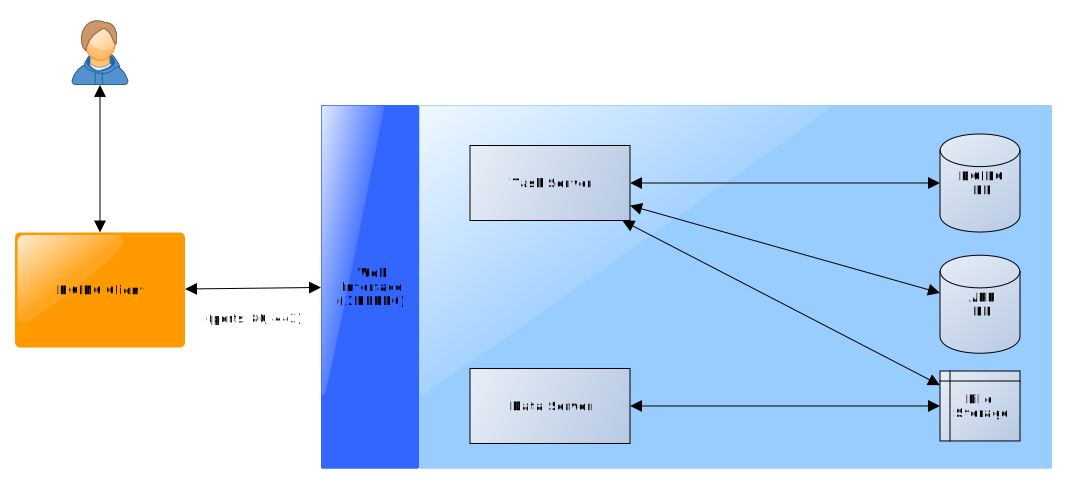
\includegraphics[width=5.5in]{images/boinc_infrastructure}
%DIFDELCMD < %%%
%DIF <  where an .eps filename suffix will be assumed under latex,
%DIF <  and a .pdf suffix will be assumed for pdflatex; or what has been declared
%DIF <  via \DeclareGraphicsExtensions.
%DIFDELCMD < \caption{%
{%DIFAUXCMD
\DIFdelFL{BOINC Architecture}}
%DIFAUXCMD
%DIFDELCMD < \label{fig:boinchla}
%DIFDELCMD < \end{figure}
%DIFDELCMD < 

%DIFDELCMD < 
%DIFDELCMD < %%%
\DIFdel{The workflow of a BOINC execution is as follows:
}%DIFDELCMD < \begin{enumerate}
\begin{enumerate}%DIFAUXCMD
%DIFDELCMD <  \item %%%
\item%DIFAUXCMD
\DIFdel{the client connects to the BOINC server (with the given credentials) and checks the status of the project. The communication is achieved using HTTP(s) (Hypertext Transfer Protocol, ports: 80 and 443) via RPC (Remote Procedure Calls), which gives access to the scheduling and processing of workunits (computations to be performed), giving tasks as (completed) results. At this point some details about BOINC nomenclature should be clarified: the name }\textit{\DIFdel{job}} %DIFAUXCMD
\DIFdel{is given to a simulation that aways into the server to be run/executed into a client and a }\textit{\DIFdel{task}} %DIFAUXCMD
\DIFdel{is a completed simulation (and its results);

}%DIFDELCMD < 

%DIFDELCMD <  \item %%%
\item%DIFAUXCMD
\DIFdel{the client asks for jobs;
 }%DIFDELCMD < \item %%%
\item%DIFAUXCMD
\DIFdel{if there are any jobs available, the server checks the client parameters (Operating System, architecture,\ldots) and the Task Server assigns and sends one to the client. For security and validation purposes each job is duplicated (and dispatched to another client as well);
 }%DIFDELCMD < \item %%%
\item%DIFAUXCMD
\DIFdel{the job is received on the client side (the required input data/files are sent by the Data Server) and the computing begins (at a lower level, a fork is done); }%DIFDELCMD < \item %%%
\item%DIFAUXCMD
\DIFdel{once the workunit is complete, the results (termed a ‘task’) are returned to the Data Server;
 }%DIFDELCMD < \item %%%
\item%DIFAUXCMD
\DIFdel{the server (internally, the validator daemon) evaluates the results, checks the integrity, and if all is correct awards credit to the client;
}
\end{enumerate}%DIFAUXCMD
%DIFDELCMD < \end{enumerate}
%DIFDELCMD < 

%DIFDELCMD < %%%
\DIFdel{In the context of CPDN a workunit is itself a member of the ensemble of climate simulations. This means that each workunit is a single and independent climate simulation.

}%DIFDELCMD < 

%DIFDELCMD < %%%
\subsection{\DIFdel{Problem Description}}

%DIFAUXCMD
\addtocounter{subsection}{-1}%DIFAUXCMD
%DIFDELCMD < 

%DIFDELCMD < %%%
\DIFdel{We now detail some of the problems that we intend to address:

}%DIFDELCMD < 

%DIFDELCMD < \begin{itemize}
%DIFDELCMD <  \item %%%
\item%DIFAUXCMD
\DIFdel{new, improved and computationally more expensive versions of the model need to be run; the }\DIFdelend \DIFaddbegin \DIFadd{there is a growing need for an on-demand and more predictable return of simulation results. A good example of this is urgent simulations for critical events in real-time (e.g., floods) where it is not possible to rely on volunteers; instead a widely available and massive scaling system is preferable (like the one described here). The }\DIFaddend current architecture and infrastructure based on BOINC  \DIFdelbegin \DIFdel{(as it is) }\DIFdelend does not provide a solution that can be scaled up for this purpose. This is because the models are running over a heterogeneous and decentralized environment (on a number of variable and different volunteers’ computers with varying configurations), where their behaviour cannot be clearly anticipated or measured, and any control over the available resources is severely limited\DIFdelbegin \DIFdel{. There is a growing need for an on-demand and more predictable solution. A good example of this is urgent simulations for critical events in real-time (e.g., floods) where it is not possible to rely on volunteers;
instead a widely available and massive scaling system is preferable (like the one described here);
 }\DIFdelend \DIFaddbegin \DIFadd{;
}

%DIF > \item a rationalization of the costs is required (and establishing useful metrics), not just for internal control but also to provide monetary quotations to project partners and funding bodies; this led us to the need of the development of a Control Plane using a system composed of a RESTful backend, using Boto to communicate with the AWS API, and SQLite3 (as a local status Database) to control the execution of the simulations, together with a frontend to display the statistics (using HTML5 and the JQuery/jqPlot libraries), information and metrics;
\DIFaddend \item \DIFdelbegin \DIFdel{regarding the previous point, there is a need to establish some kind of metrics;
 }%DIFDELCMD < \item %%%
\item%DIFAUXCMD
\DIFdelend a rationalization of the costs is required \DIFaddbegin \DIFadd{(and establishing useful metrics)}\DIFaddend , not just for \DIFdelbegin \DIFdel{self-control }\DIFdelend \DIFaddbegin \DIFadd{internal control }\DIFaddend but also to provide monetary quotations to project partners and funding bodies; \DIFdelbegin %DIFDELCMD < \end{itemize}
%DIFDELCMD < 
%%%
\DIFdelend \DIFaddbegin \DIFadd{this led us to the need of the development of a Control Plane together with a frontend to display the statistics information and metrics;
}\DIFaddend 

\DIFdelbegin \DIFdel{For these reasons we propose to implement the following:
}%DIFDELCMD < \begin{itemize}
%DIFDELCMD <  %%%
\DIFdelend \item \DIFdelbegin \DIFdel{full conversion of the model to an Infrastructure as a Service (IaaS)~\mbox{%DIFAUXCMD
\citep{armbrust2010view}}%DIFAUXCMD
, by migration into a Cloud Infrastructure (Amazon Web Services (AWS)~\mbox{%DIFAUXCMD
\citep{cloud2011amazon}}%DIFAUXCMD
), including computing and (shared) storage resources;
 }%DIFDELCMD < \item %%%
\item%DIFAUXCMD
\DIFdel{Implementation of a Central Control System (including a Dashboard) that will manage the distribution of tasks, as well as displaying high-level metrics and statistics for the different project actions and deployments;
}%DIFDELCMD < \item %%%
\item%DIFAUXCMD
\DIFdel{Use }\DIFdelend \DIFaddbegin \DIFadd{use }\DIFaddend of Free Software in order to promote scientific reproducibility\DIFdelbegin \DIFdel{\mbox{%DIFAUXCMD
\citep{anel2011}}%DIFAUXCMD
;
 }\DIFdelend \DIFaddbegin \DIFadd{~\mbox{%DIFAUXCMD
\citep{anel2011}}%DIFAUXCMD
;
}

\DIFaddend \item \DIFdelbegin \DIFdel{Complete }\DIFdelend \DIFaddbegin \DIFadd{complete }\DIFaddend documentation of the process\DIFdelbegin \DIFdel{;
}\DIFdelend \DIFaddbegin \DIFadd{, allowing knowledge to be transferred or migrated easily to other systems~\mbox{%DIFAUXCMD
\citep{montes2014}}%DIFAUXCMD
. Additional explanations can be found in the appendices (Appendix A, Appendix B and Appendix C).
}\DIFaddend \end{itemize}

\DIFaddbegin \DIFadd{Furthermore, in this work we wish to prove the feasibility of running complex applications in this environment. We use weather@home~\mbox{%DIFAUXCMD
\citep{massey2015}}%DIFAUXCMD
, a high resolution regional climate model nested in a global climate model as an example. The remainder of this paper is organized as follows. We firstly present benchmarks of the weather@home application run in AWS, in section~\ref{section:benchmarks}, then describe the migration of the CPDN infrastructure to AWS in section~\ref{section:cpdn_infrastructure}. We also describe our control plane in section~\ref{section:control_plane} to conduct the simulations and manage the cloud resources. Lastly the results are discussed in the conclusion.
}

\DIFaddend \section{BOINC deployment to the Cloud}

\DIFdelbegin \DIFdel{The proposal presented here has been built using }\DIFdelend \DIFaddbegin \subsection{\DIFadd{Application benchmarks in Amazon Web Services (AWS)}}
\label{section:benchmarks}

\DIFadd{The example presented here is running CPDN in }\DIFaddend AWS. AWS is the largest Infrastructure as a Service (IaaS) provider, it is very well documented\DIFdelbegin \DIFdel{and is sufficiently "open" to easily allow migration from and to other Clouds}\DIFdelend , as well as being the most suitable solution for the problem at present (and with fewer limitations than other providers).

The first step was to \DIFdelbegin \DIFdel{estimate the size of the problem, in this case for CPDN specifically, therefore test runs were carried out using different and representative }\DIFdelend \DIFaddbegin \DIFadd{benchmark different }\DIFaddend AWS EC2 \DIFdelbegin \DIFdel{types of instances. Two systems (EC2 instance type) were evaluated for this: The m1.large instance type, that  was intended for general purpose computation, with a 64-bit processor (}\DIFdelend \DIFaddbegin \DIFadd{instance types}\footnote{\DIFadd{https://aws.amazon.com/ec2/instance-types/}} \DIFadd{to determine their performance running CPDN simulations. These tests were done with a range of instance types, but only choosing instance types that have HMV virtualization available. EBS gp2 storage}\footnote{\DIFadd{http://docs.aws.amazon.com/AWSEC2/latest/UserGuide/EBSVolumeTypes.html}} \DIFadd{was used for all instances for ease of comparison. These tests were carried out running multiple copies of a single workunit, in parallel, with the number of simulations matching the number of vCPUs (hyperthreads) available to each instance type. For each instance's types at least 4 tests were run.
}

\DIFadd{For benchmarking purposes, short 1 day climate simulations were run.  The model used here is weather@home2 (atmosphere only model HadAM3P~\mbox{%DIFAUXCMD
\citep{gordon2000}}%DIFAUXCMD
, driving the regional version of the same model, HadRM3P~\mbox{%DIFAUXCMD
\citep{pope2000}}%DIFAUXCMD
). This version of the model uses the MOSES }\DIFaddend 2 \DIFdelbegin \DIFdel{vCPUs), 7.5 GB of RAM and 2 x 420GB storage units (identified as }\textit{\DIFdel{System \#1}} %DIFAUXCMD
\DIFdel{into  Figure \ref{fig:plot_time_cost}) and the cg1.4xlarge instance , used for intensive computation (CPU and GPU) with a 64-bit processor (16 vCPUs), 24 GB of RAM, 2 x 840GB storage units and 2 x Tesla M-Class M2050 GPUs (identified as }\textit{\DIFdel{System \#2}} %DIFAUXCMD
\DIFdel{into Figure \ref{fig:plot_time_cost}) . 
m1.large was selected because it was the more efficient typefor this problem (when performing these tests) thanks to a better price per workunit, as can be seen in Figure \ref{fig:plot_time_cost}.

}\DIFdelend \DIFaddbegin \DIFadd{land surface scheme. The region chosen is at 0.22 degree ($\approx$ 25 km) resolution over Europe.
}\DIFaddend 

\DIFdelbegin \DIFdel{Some aspects of the problem were also drafted thanks to these runs: CPU usage was always between 98\% and 100\%, memory usage was residual (average: 1.5\%), GPUs could not be checked for improvement in terms of performance (because they were not supported when our experiments were executed) , scratch storage was low, and some parts of the code still ran in 32bit mode}\DIFdelend %DIF > Some aspects of the problem were also drafted thanks to these runs: CPU usage was always between 98\% and 100\%, memory usage was residual (average: 1.5\%), GPUs could not be checked for improvement in terms of performance (because they were not supported when our experiments were executed), scratch storage was low, and some parts of the code still ran in 32bit mode.
\DIFaddbegin 

\DIFadd{Figure \ref{fig:plot_time_cost}a shows the average time to run all of the simulations on a particular instance, by instance type. We see a general trend of smaller instances performing better than larger instances. This is likely due to the hardware these instances are on being at a lower load. Running only a single simulation per instance resulted in similar run times for instances of the same category (e.g. c4), and they are not shown in the figure. However, we have verified that it is more cost effective to run the maximum number of simulations per instance than to run instances at a lower load.
}

\DIFadd{Figure \ref{fig:plot_time_cost}b shows the estimated cost of running a one year simulation on each each instance type. The pricing here is based on the Spot Price}\footnote{\DIFadd{https://aws.amazon.com/ec2/spot/pricing/}} \DIFadd{in the cheapest availability zone in the us-east-1 region  as of June 2016. This shows that the current generation compute optimized instances (c4) had three out of the four most cost effective choices, but other small instance types are amongst the cheapest. We emphasise that these results are very variable in time and between regions. In the us-west-1 region and us-west-2 regions, the cheapest instance types were m4.large and m4.xlarge respectively, due to the lower spot price for those particular instances in those regions}\DIFaddend .


\begin{figure}[!h]
\centering
\DIFdelbeginFL %DIFDELCMD < \includegraphics[width=4.5in]{images/plots/plot_time}
%DIFDELCMD < \includegraphics[width=4.5in]{images/plots/plot_costs}
%DIFDELCMD < %%%
\DIFdelendFL \DIFaddbeginFL \includegraphics[width=6.5in]{images/plot_time_cost}
\DIFaddendFL \caption{\DIFaddbeginFL \DIFaddFL{a) }\DIFaddendFL Workunit \DIFdelbeginFL \DIFdelFL{Processing Time }\DIFdelendFL \DIFaddbeginFL \DIFaddFL{run time }\DIFaddendFL and \DIFdelbeginFL \DIFdelFL{Simulation }\DIFdelendFL \DIFaddbeginFL \DIFaddFL{b) }\DIFaddendFL Cost \DIFaddbeginFL \DIFaddFL{per simulation year}\DIFaddendFL .}
\label{fig:plot_time_cost}
\end{figure}


\subsection{\DIFdelbegin \DIFdel{Climateprediction.net as an example}\DIFdelend \DIFaddbegin \DIFadd{CPDN infrastructure in AWS}\DIFaddend }
\DIFaddbegin \label{section:cpdn_infrastructure}
\DIFaddend 

Based on the previous tests, new infrastructure was designed on the cloud (Figure \ref{fig:cloudinfra}). Several steps were required for its implementation, as described below.

\DIFdelbegin %DIFDELCMD < \begin{figure}[!h]
%DIFDELCMD < %%%
\DIFdelendFL \DIFaddbeginFL \begin{figure}[h!]
\DIFaddendFL \centering
\includegraphics[width=6.5in]{images/cloud_infrastructure}
\caption{Proposed Cloud Infrastructure}
\label{fig:cloudinfra}
\end{figure}


\subsubsection{Computing Infrastructure}
\begin{enumerate}
\item First of all a template was created to allow automated instance creation including:

\begin{itemize}
	%DIF > \item instance selection: AWS m1.large;
	\item instance \DIFdelbegin \DIFdel{Selection: AWS m1.large}\DIFdelend \DIFaddbegin \DIFadd{selection, based on the benchmarks presented in section~\ref{section:benchmarks}}\DIFaddend ;
	\item base operating system installation: Amazon Linux (64 bit) was used for this \DIFdelbegin \DIFdel{document}\DIFdelend \DIFaddbegin \DIFadd{work}\DIFaddend ;
	\item storage definition: 16~GB, persistent, standard EBS for this case;
        \item firewall configuration: inbound only SSH(22) accepted, outbound everything accepted;
        \item installation and configuration of BOINC client inside the template image, including its dependencies such as \DIFdelbegin \DIFdel{32bit }\DIFdelend \DIFaddbegin \DIFadd{32 bit }\DIFaddend libraries. It is recommended to use the latest version from git;%DIF > ~\citep{git};

\end{itemize}

\item \DIFdelbegin \DIFdel{contextualization of the template: this part is strongly related to the Cloud system type}\DIFdelend \DIFaddbegin \DIFadd{instance contextualization: post installation configuration}\DIFaddend , for example in AWS this is achieved by creating a machine image (AMI) and adjusting it by selecting the appropriate options such as the Kernel image (AKI);
\item (optional) installation and configuration of AWS EC2 Command Line interface. This can be useful to debug or troubleshoot issues with the infrastructure;


\end{enumerate}

\subsubsection{Storage Infrastructure}
Another problem that needs \DIFdelbegin \DIFdel{solving is the scarcity of storage space as well as its centralization (in the University of Oxford) in the current infrastructure, given than }\DIFdelend \DIFaddbegin \DIFadd{to be solved is the need for a decentralized, low-latency and world-wide accessible storage for the output data (}\DIFaddend each simulation (36000 workunits) generates $\sim$656~GB of results\DIFaddbegin \DIFadd{)}\DIFaddend . A solution for this could be a distributed (accessed within different and synchronized world-wide endpoints) and scalable massive storage (Figure \ref{fig:storage}). Here we tested an architecture in which the clients send the results (tasks) to an Amazon Simple Storage Service (S3) bucket (storage endpoint). At the same time\DIFdelbegin \DIFdel{the }\DIFdelend \DIFaddbegin \DIFadd{, }\DIFaddend CPDN can access these data over the internet to run postprocessing (e.g., a custom assimilator); this can be achieved using the AWS API.

\begin{figure}[!h]
\centering
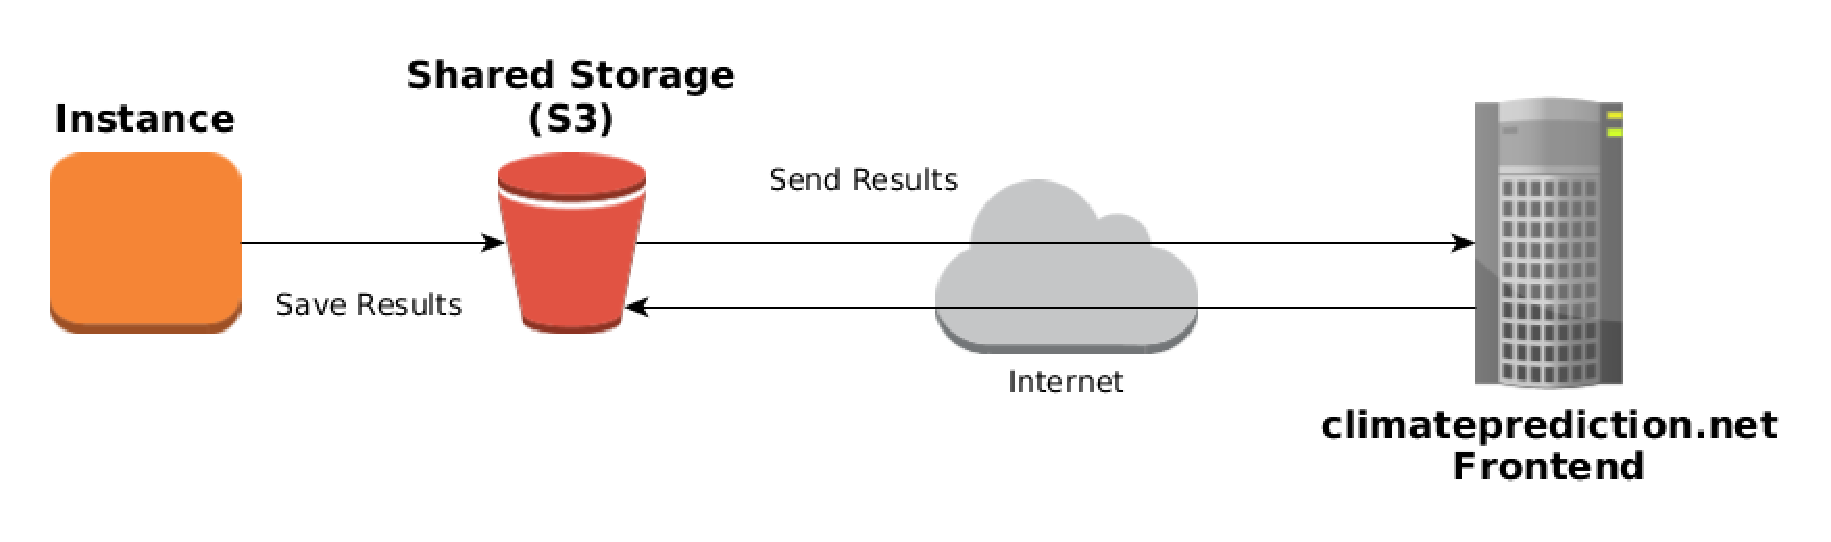
\includegraphics[width=4.5in]{images/storage_architecture}
\caption{Shared Storage Architecture}
\label{fig:storage}
\end{figure}

\DIFdelbegin \subsubsection{\DIFdel{Project Control Plane}}

%DIFAUXCMD
\addtocounter{subsubsection}{-1}%DIFAUXCMD
\DIFdelend \DIFaddbegin \DIFadd{Given this values, every workunit returns a result of $\sim$0.018~GB with a price of $\sim$USD0.005414 each ~\mbox{%DIFAUXCMD
\citep{S3pricing}}%DIFAUXCMD
, and $\sim$USD194.904 for the full simulation (both storage and data transfer).
}\DIFaddend 

\DIFaddbegin \subsection{\DIFadd{Project Control Plane}}

\label{section:control_plane}

\DIFaddend Having set up the computing and storage infrastructure, we still lack a control plane to provide \DIFdelbegin \DIFdel{an extra }\DIFdelend \DIFaddbegin \DIFadd{a }\DIFaddend layer for abstraction and automation, and providing more consistency to the project. The aim of developing the Central Control System (Figure \ref{fig:dashboard_architecture}) is to provide a Cloud-agnostic\DIFdelbegin \DIFdel{and an }\DIFdelend \DIFaddbegin \DIFadd{, }\DIFaddend easy-to-use frontend (Figure \ref{fig:dashboard}) to manage the experiments with minimal knowledge of the underlying architecture and obtain a real-time overview of the current status (including the resources used and run completion data). Moreover, the Central Control System lends more consistency to the view of the project as an IaaS by providing a simple interface (both backend and frontend).

The Control Plane is still in its early developmental stages (e.g., although it is cloud-agnostic, so far only AWS has a connector and is supported), and further work will describe its improvements over time.

It consists of two main components:

\begin{itemize}
 \item backend: this provides the user with a RESTful API with basic functionalities related to simulation information and management, with the intention of providing (even more) agnostic access to the Cloud;
 \item frontend: this makes it easier to communicate with the API as intuitively and simplistically as possible;
\end{itemize}

 The core component\DIFdelbegin \DIFdel{is }\DIFdelend \DIFaddbegin \DIFadd{, }\DIFaddend the RESTful backend (using JSON)\DIFdelbegin \DIFdel{that }\DIFdelend \DIFaddbegin \DIFadd{, }\DIFaddend provides simple access and wraps common actions: start simulation with n-nodes, stop simulation, modify simulation parameters (n-nodes), get simulation status, and get simulation metrics.


\begin{figure}[!h]
\centering
\includegraphics[width=6.5in]{images/dashboard_architecture}
\caption{Dashboard and metrics application architecture}
\label{fig:dashboard_architecture}
\end{figure}

\begin{figure}[!h]
\centering
\DIFdelbeginFL %DIFDELCMD < \includegraphics[width=6.5in]{images/screenshots/gui/dashboard01.eps}
%DIFDELCMD < %%%
\DIFdelendFL \DIFaddbeginFL \includegraphics[width=6.5in]{images/screenshots/gui/dashboard01}
\DIFaddendFL \caption{Dashboard}
\label{fig:dashboard}
\end{figure}

\DIFdelbegin \subsubsection{\DIFdel{Full Infrastructure Runs}}
%DIFAUXCMD
\addtocounter{subsubsection}{-1}%DIFAUXCMD
\DIFdel{Finally, we performed several experiments using regular simulations (workunits) }\DIFdelend \DIFaddbegin \begin{conclusions}
\DIFadd{Several experiments (using all the defined infrastructure) were done by using standard workunits }\DIFaddend developed by the climateprediction.net/weather\@home project\DIFdelbegin \DIFdel{\mbox{%DIFAUXCMD
\citep{massey2014}}%DIFAUXCMD
}\DIFdelend . We processed workunits from two main experiments: the weather\@home UK floods\DIFdelbegin \DIFdel{\mbox{%DIFAUXCMD
\citep{weatherhome2014} }%DIFAUXCMD
}\DIFdelend \DIFaddbegin \DIFadd{~\mbox{%DIFAUXCMD
\citep{schaller2016} }%DIFAUXCMD
}\DIFaddend and the weather\@home Australia New Zealand project\DIFdelbegin \DIFdel{. Both experiments rely for their simulations of the atmosphere only on the general circulation model HadAM3P \mbox{%DIFAUXCMD
\citep{gordon2000}}%DIFAUXCMD
, which drives the regional version of the same model, HadRM3P \mbox{%DIFAUXCMD
\citep{pope2000}}%DIFAUXCMD
. The }\DIFdelend \DIFaddbegin \DIFadd{~\mbox{%DIFAUXCMD
\citep{black2016}}%DIFAUXCMD
, both with an }\DIFaddend horizontal resolution of \DIFdelbegin \DIFdel{these simulations was }\DIFdelend 50 km.
\DIFdelbegin \DIFdel{The outputs of the workunits for the weather}%DIFDELCMD < \@%%%
\DIFdel{home UK floods experiment were previously successfully described in two other research papers \mbox{%DIFAUXCMD
\citep{schaller2014,anel2014}}%DIFAUXCMD
.

}\DIFdelend 

\DIFdelbegin %DIFDELCMD < \begin{conclusions}
%DIFDELCMD < %%%
\DIFdelend It has been successfully demonstrated that it is possible to run simulations of a climatic model using infrastructure in the Cloud; while this might not seem complex, to the best of our knowledge it has never previously been tested. This efficient use of MTC resources for scientific computing has previously been used to facilitate real research in other areas\DIFaddbegin \DIFadd{~}\DIFaddend \citep{anel2014, schaller2014}.

\DIFdelbegin \DIFdel{Even though a better performance was achieved using the AWS cg1.4xlarge instance (Figure \ref{fig:plot_time_cost}), on analyzing the data it would appear that m1.large was more efficient because the price per workunit is better and the average time per workunit is still less than the current one obtained by CPDN under the normal BOINC deployment using volunteer computing ($\sim$7 days/workunit vs.\ $\sim$8 days/workunit). The new version is therefore more suitable for simulations . In any case, prices and specifications may vary within a short time and this would be different for other Cloud services, implying that an automated re-evaluation of the ratio of workunits/hour price may be necessary (prices for this evaluation were last determined on 10/06/2014)}\DIFdelend \DIFaddbegin \DIFadd{We have benchmarked a number of Amazon EC2 instance types running CPDN workunits. Prices for spot instances vary significantly over time and between instance, but we estimate a price as low as \$1.50 to run a one year simulation based on the c4.large instance in the us-west-1 region in June 2016 (see Figure~\ref{fig:plot_time_cost}). To optimise the costs of running simulations in this environment it will be important to automatically re-evaluate the spot prices to choose the cheapest instance type at the time simulations are submitted}\DIFaddend .

It is interesting to note that Cloud services enable us to achieve a given number of tasks completed in some cases five times faster than using the regular volunteer computing infrastructure. However, the financial implications can only be justified for critical cases where stakeholders \DIFdelbegin \DIFdel{need the results of the simulations regardless of cost. }\DIFdelend \DIFaddbegin \DIFadd{are able to jusity through a specific cost benefit analysis.
}\DIFaddend 

\DIFaddbegin \DIFadd{About our usage and solution for storage: S3 was a good fit for our needs (it comes out-of-the box with AWS and the pricing is convenient) but we understand that, even though the infrastructure here described cover a good number of use cases for different projects and experiments, other alternatives could be analysed:
}

\begin{itemize}
 \item \DIFadd{AWS Glacier is an interesting option to study in case that long-term, for non-immediate access and with lower-cost, storage for data is needed ~\mbox{%DIFAUXCMD
\citep{AWSGlacier}}%DIFAUXCMD
. In our case a full simulation (36000 workunits) would have costed us USD2.624 per month of storage.  
 }\item \DIFadd{S3 file size is limited to 5TB and this could be a problem for bigger projects so, options like a CephFS cluster on EC2 could be interesting ~\mbox{%DIFAUXCMD
\citep{zhao2015}}%DIFAUXCMD
.
}

\end{itemize}

\DIFaddend This research has also served as a basis for obtaining new research \DIFdelbegin \DIFdel{projects }\DIFdelend \DIFaddbegin \DIFadd{funding }\DIFaddend as part of climateprediction.net \DIFdelbegin \DIFdel{, in particular a project led by one of the co-directors of the thesis achieved in May of this year the Microsoft Azure for Research Award \mbox{%DIFAUXCMD
\citep{azure2014}}%DIFAUXCMD
, one of only about 200 projects funded by Microsoft Research, for }\DIFdelend \DIFaddbegin \DIFadd{for }\DIFaddend state-of-art studies using Cloud Computing technologies. This project is based on demonstrated successes in the application of technologies and solutions of the type described here.

In summary, the achieved high-level objectives were:
\begin{itemize}
 \item the client side was successfully migrated to the Cloud (EC2\DIFdelbegin \DIFdel{+S3}\DIFdelend );

 \item \DIFaddbegin \DIFadd{the upload server capability was configured to be redirected to AWS S3 buckets;
}

 \item \DIFaddend different simulations were successfully run over the new infrastructure;

 \item a Control Plane (including a Dashboard: frontend and backend) was developed, deployed and tested;

 \item a comprehensive costing of the project and the simulation were obtained, together with metrics;
\end{itemize}

Future improvements should focus on providing more logic to the interaction with client status (\DIFdelbegin \DIFdel{probably via }\DIFdelend \DIFaddbegin \DIFadd{such as through }\DIFaddend RPC calls) allowing more metrics to be pulled from them\DIFdelbegin \DIFdel{and perhaps }\DIFdelend \DIFaddbegin \DIFadd{, and }\DIFaddend creating new Software as a Service (a SaaS layer). From the infrastructure point of view, two main improvements are possible: first, a probe/dummy automated execution will be needed to adjust the price to a real one before each simulation; second, full migration of the server side into the Cloud, allowing the costs of data transfer and latency to be dramatically reduced.

\hfill \break
\end{conclusions}

\authorcontribname. All the authors participated into the design of the experiments and the analysis of results. D. Montes implemented the \DIFdelbegin \DIFdel{experiments. }\DIFdelend \DIFaddbegin \DIFadd{full infrastructure experiments. P. Uhe carried out the benchmarking. }\DIFaddend All authors participated in the writing of this paper.

\begin{acknowledgements}
We thank Andy Bowery, Jonathan Miller and Neil R. Massey for all their help and assistance with the internals and specifics of the CPDN BOINC implementation. \DIFaddbegin \DIFadd{We also thank the comments by B. N. Lawrence, C. Fernández and A. Arribas that have helped to improve this paper. The compute resources for this project were provided under the AWS Cloud Credits for Research Program.
}\DIFaddend 

\end{acknowledgements}

%% REFERENCES

%% The reference list is compiled as follows:

%\begin{thebibliography}{}

%\bibitem[AUTHOR(YEAR)]{LABEL}
%REFERENCE 1

%\bibitem[AUTHOR(YEAR)]{LABEL}
%REFERENCE 2

%\end{thebibliography}

%% Since the Copernicus LaTeX package includes the BibTeX style file copernicus.bst,
%% authors experienced with BibTeX only have to include the following two lines:
%%
\bibliographystyle{copernicus}
\bibliography{1_general.bib}
\DIFaddbegin 


\appendix
\section{\DIFadd{Computing Infrastructure Design and Implementation}}

\DIFadd{The new computing infrastructure was built over virtualized instances (AWS EC2). Amazon provides also Autoscaling Groups that allow the user to define policies to add or remove dynamically instances triggered by a defined metric or alarm. As the purposes of this work are to use the rationalization of the resources and to have full control over them (via the Central System), as well as any type of Load Balancing or Failover, this feature will not be used in the Cloud side but in the control system node that serves as backend for the Dashboard.
}

%DIF > \noindent The new workflow for a project/model execution is:

%DIF > Prerequisites: tasks have been setup in the server side and are ready to be sent to the clients, this can be currently checked into the public URL \url{http://climateapps2.oerc.ox.ac.uk/cpdnboinc/server_status.html}


\DIFadd{After tasks have been setup in the server side and are ready to be sent to the clients (this can be currently checked into the public URL
}\url{http://climateapps2.oerc.ox.ac.uk/cpdnboinc/server_status.html}\DIFadd{), the new workflow for a project/model execution is:
}

\begin{enumerate}
 \item \DIFadd{The (project) administrator user configures and launches a new simulation via the Dashboard.
 }\item \DIFadd{The required number of instances are created based on a given template that contains a parametrized image of GNU/Linux with a configured BOINC client.
 }\item \DIFadd{Every instance connects to the server and fetchs 2 tasks (1 per CPU, as the used instances have 2 CPU).
 }\item \DIFadd{When a task is processed, the data will be returned to the server, and also stored into a Shared Storage so it will be accessible for a given set of authorized users.
 }\item \DIFadd{Once there are not tasks available, the Control Node will shut down the instances.
}\end{enumerate}

\DIFadd{It should be noted that, at any point, the administrator will be able to have real time data about the execution (metrics, costs...) as well as change the running
parameters and apply them over the infrastructure.
}

\subsection{\DIFadd{Template Instance Creation}}

\DIFadd{In order to be able to create an homogeneous infrastructure the first step is to create an (EC2) instance that can be used as template for the other ones.
}

\begin{table}[h!]
%DIF > \begin{center}
\begin{tabular}{|l|l|}
\hline\hline
\DIFaddFL{OS Image (AMI): }& \DIFaddFL{Amazon Linux AMI 2014.03.1 (64 bit)}\\ \hline
\DIFaddFL{Instance Type: }& \DIFaddFL{m1.large}\\ \hline
\DIFaddFL{Firewall (Security Groups): }& \DIFaddFL{Inbound: Only SSH (22) Accepted}\\
\DIFaddFL{\mbox{} }& \DIFaddFL{Outbound: Everything Accepted.}\\ \hline
\DIFaddFL{Persistent Storage: }& \DIFaddFL{Root 16GB (volume type: standard)}\\ \hline\hline
\end{tabular}
\caption{\DIFaddFL{Parameter for the template instances}}
\label{table:templateInstanceSpecs}
%DIF > \end{center}
\end{table}

\DIFadd{The high level steps to follow to get a Template Instance (with the parameters defined in the Table~\ref{table:templateInstanceSpecs}) are exposed below:
}\begin{enumerate}

\item \DIFadd{On the AWS dashboard click ``Launch Instance'', then select the given OS image (AMI) type.
  }\begin{center}
  \includegraphics[width=2.5in]{images/screenshots/instance_creation/01.png}\\
  \includegraphics[width=6.5in]{images/screenshots/instance_creation/02.png}
  \end{center}


\item \DIFadd{Select the image type .
  }\begin{center}
  \includegraphics[width=2.5in]{images/screenshots/instance_creation/03.png}\\
  \includegraphics[width=6.5in]{images/screenshots/instance_creation/04.png}
\end{center}

\item \DIFadd{Revise and set the parameters:
}\begin{center}
  \includegraphics[width=3.5in]{images/screenshots/instance_creation/05.png}\\
  \includegraphics[width=4.5in]{images/screenshots/instance_creation/06.png}\\
  \includegraphics[width=6.5in]{images/screenshots/instance_creation/07.png}\\
\end{center}

\item \DIFadd{Launch the Template Instance.
}

\end{enumerate}

\DIFadd{Note: remember to create a new keypair (public-private key used for passwordless SSH access to the instances) and save it (it will be used for the Central System), or use another one that already exists and is currently accessible. Because of the limited space into this article the line length (new line) has been truncated with $\backslash$, please consider this when running any command described in here.
}

\subsubsection{\DIFadd{Installing and testing AWS and EC2 Command-Line Interface}}

\DIFadd{(Prerequisites: wget, unzip and Python 2.7.x)
}

\DIFadd{This step is optional, but it is highly recommendable because this will be advanced control of the infrastructure through the shell.
The follow description applies and have been tested on Ubuntu 14.04~\mbox{%DIFAUXCMD
\cite{ubuntu}}%DIFAUXCMD
, but can be reproduced into any GNU/Linux system:
}

\DIFadd{First, create an }\textit{\DIFadd{Access Key}} \DIFadd{(and secret/password), via the AWS web interface in the }\textit{\DIFadd{Security Credentials}} \DIFadd{section. With this data the }\textit{\DIFadd{AWS\_ACCESS\_KEY}} \DIFadd{and
}\textit{\DIFadd{AWS\_SECRET\_KEY}} \DIFadd{variables should be exported/updated, please have in mind that this mechanism will be also used for the Dashboard/Metrics Application:
}

\begin{verbatim}
$ echo "export AWS_ACCESS_KEY = \
<your-aws-access-key-id>" \
>> $HOME/.bashrc
$ echo "export AWS_SECRET_KEY = \
<your-aws-secret-key>" \
>> $HOME/.bashrc

$ source $HOME/.bashrc
\end{verbatim}

\begin{verbatim}
#Download and install the AWS CLI
$ wget https://s3.amazonaws.com/\
aws-cli/awscli-bundle.zip &&\
unzip awscli-bundle.zip &&\
sudo ./awscli-bundle/install -i \
/usr/local/aws -b /usr/local/bin/aws

#Download EC2 API tools
wget http://s3.amazonaws.com/\
ec2-downloads/ec2-api-tools.zip &&\

sudo mkdir /usr/local/ec2 &&\
sudo unzip ec2-api-tools.zip -d \
/usr/local/ec2

#Remember to update the
#PATH=$PATH:/usr/local/ec2/\
#ec2-api-tools-<API_VERSION>/bin
$ echo "export JAVA_HOME=/usr/lib/jvm\
/java-6-openjdk-amd64/" >>
$HOME/.bashrc

$ source $HOME/.bashrc
\end{verbatim}

\subsubsection{\DIFadd{Installing BOINC and its dependencies}}

\DIFadd{The project executes both 32 and 64 bits binaries for the simulation so once the Template Instance is running, the needed packages and dependencies need to be installed via:
}

\begin{verbatim}
$ sudo yum install expat.i686 flac.i686 \
fontconfig.i686 freetype.i686 gamin.i686 \
glib2.i686 glibc.i686gnutls.i686 \
gtk2.i686 libX11.i686 libXau.i686 \
libXext.i686 libXfixes.i686  libXft.i686 \
libXi.i686 libcom_err.i686 libgcc.i686 \
libgcrypt.i686 libgpg-error.i686 \
libstdc++.i686 libxcb.i686 xcb-util.i686 \
zlib.i686 libcurl.i686 openssl097a.i686
\end{verbatim}


\DIFadd{The version of BOINC used will be the latest from git~\mbox{%DIFAUXCMD
\citep{git}}%DIFAUXCMD
. To download and compile it:
}

\begin{verbatim}
#Install needed development tools
$ sudo yum groupinstall 'Development Tools'

$ sudo yum install git libcurl \
libcurl-devel openssl097a.i686 \
openssl-devel

#Fetch BOINC source code, compile and
#install the client
$ git clone \
git://boinc.berkeley.edu/boinc-v2.git \
boinc && cd boinc && ./_autosetup \
&& ./configure --disable-server \
--disable-manager --enable-optimize \
&& make \
&& sudo make install

#Create user and set permissions and
#ownership
#(in case that we want a boinc user)
$ sudo adduser boinc
$ sudo chown boinc /var/lib/boinc
\end{verbatim}

\DIFadd{Once the BOINC client is installed it must be configured so it will automatically run on every instance
with the same parameters:}\\

\begin{enumerate}

 \item  \DIFadd{Create a new account in the project:
}

\begin{verbatim}
$ boinccmd --create_account \
climateprediction.net <EMAIL> \
<PASSWORD> <NAME>
\end{verbatim}


\item \DIFadd{With the account created (or if already done) the client needs to be associated to the project by
creating a configuration file with the user token:
}

\begin{verbatim}
$ boinccmd --lookup_account \
climateprediction.net <EMAIL> \
<PASSWORD>| grep "account key" \
| sed 's/\(.*\): \(.*\)/\2/g' \
| xargs boinccmd --project_attach \
climateprediction.net

#Status check
$ boinccmd --get_state
\end{verbatim}

\item \DIFadd{Make BOINC to start with the system (ec2-user will be used because of permissions):
}

\begin{verbatim}
$sudo echo 'su - ec2-user -c \
"cd /home/ec2-user/boinc-client/\
bin/ && ./boinc --daemon"'\
>> /etc/rc.local
\end{verbatim}

\end{enumerate}

\subsubsection{\DIFadd{Simulation Terminator}}

\DIFadd{An essential piece of software, developed for this work, is the }\textit{\DIFadd{Simulation Terminator}}\DIFadd{, that decides if a node should shutdown itself in case that workunits were not processed for a given amount of time (by default 6 hours, via cron) or there are no jobs waiting on the server.
}

\DIFadd{This application will be provided upon request to the authors.
}


\DIFadd{To install it (by default into }\textit{\DIFadd{/opt/climateprediction/}} \DIFadd{):
}

\begin{verbatim}
$ sudo ./installClient
>> Simulation Client succesfully installed!
\end{verbatim}

\DIFadd{When an instance is powered off, it will be terminated (destroyed) by the }\textit{\DIFadd{Reaper}} \DIFadd{service, that runs into the Central Control System.
}


\subsection{\DIFadd{Contextualization}}

\DIFadd{Now that the Template Instance is ready, this is that all the parameters have been configured and the BOINC client is ready to start processing tasks, the next stage is to contextualize it. This means that a OS image will be created from it, which will give our infrastructure the capacity of being scalable by creating new instances from this new image. Unfortunately this part is strongly related with the Cloud type, and although can be replicated into another systems, by now it will only explicitly work in this way for AWS.
}

\DIFadd{The steps to follow:
}\begin{enumerate}
 \item \DIFadd{On the instances list (AWS Dashboard), select the Template Instance, right click and select }\textit{\DIFadd{Create Image}}\DIFadd{,
 name of the image: }\textit{\DIFadd{CLIMATE\_PREDICTION\_TEMPLATE}}\DIFadd{. This will create a disk Image that can be used for a full Instance Template (AMI):
}\begin{center}
  \includegraphics[width=4.5in]{images/screenshots/image_creation/01.png} \\
  \includegraphics[width=6.5in]{images/screenshots/image_creation/02.png}
\end{center}

\item \DIFadd{To finally create the Instance Image (in the AWS Dashboard) go to Ima\-ges$\rightarrow$AMIs and right click on }\textit{\DIFadd{CLIMATE\_PREDIC\-TION\_TEMPLATE}}
 \DIFadd{and fill the parameters, at least name as }\textit{\DIFadd{CLIMATE\_PREDICTION\_TEMPLATE}} \DIFadd{(the same as Image, for better identification) and match the kernel image (AKI) with the original
 Template Instance (currently: aki-919dcaf8). This step is very important, otherwise the new instances created for the project simulations
 won't boot correctly.
}\begin{center}
  \includegraphics[width=4.5in]{images/screenshots/image_creation/03.png}\\
  \includegraphics[width=6.5in]{images/screenshots/image_creation/04.png}
\end{center}
\end{enumerate}

\DIFadd{At this point the Computing infrastructure is ready to be deployed and scaled, this will be done trough the Dashboard.
}


\section{\DIFadd{Upload Server}}

\DIFadd{Once a client has processed a workunit, the task (result) is created and sent to the defined Upload Server, that for the CPDN is }\url{http://cpdn-upload2.oerc.ox.ac.uk/cpdn_cgi/file_upload_handler}\DIFadd{. This needs to be done in a transparent way for the clients and without modifying the server because we don't want to affect the actual running experiments (but in the future the servers should distribute a configuration that directly points to the S3 bucket). To do this the data should be intercepted, and this can be done in 2 steps/components:
}


\begin{itemize}
 \item \textbf{\DIFadd{The name resolution}} \DIFadd{should be }\textit{\DIFadd{faked}} \DIFadd{by changing the CNAME }\url{http://cpdn-upload2.oerc.ox.ac.uk/cpdn_cgi/file_upload_handler} \DIFadd{point to the created S3 bucket endpoint. Bind documentation can be reviewed for this in~\mbox{%DIFAUXCMD
\cite{bind2010}
}%DIFAUXCMD
}

\item \textbf{\DIFadd{A web server as endpoint}}\DIFadd{, with HTTP and HTTPs support, configured to resolve the URL }\url{http://$UPLOAD_SERVER/cpdn_cgi/} \DIFadd{(the jobs are created to target this URL). To simplify this stage, the storage provided by AWS, S3, will be used because it has a simple HTTP(s) server that supports all the required HTTP methods (GET and POST). The (expected) content of the }\textit{\DIFadd{file\_upload\_handler}} \DIFadd{must be:
}

\begin{verbatim}
<data_server_reply>
    <status>1</status>
</data_server_reply>
\end{verbatim}

\begin{enumerate}
\item \DIFadd{Access to the S3 Service from the AWS dashboard.
}\begin{center}
  \includegraphics[width=2.1in]{images/screenshots/storage/storage01.png}
\end{center}

\item \DIFadd{Click on "Create" Bucket, the name should be }\textit{\DIFadd{CLIMATE\_PREDICTION}} \DIFadd{and must be in the same Region than the instances.
}\begin{center}
  \includegraphics[width=4.5in]{images/screenshots/storage/storage02.png}
\end{center}

\item \DIFadd{Activate (in the Options) the HTTP/HTTPs server.
}\begin{center}
  \includegraphics[width=4.5in]{images/screenshots/storage/storage03.png}\\
  \includegraphics[width=4.5in]{images/screenshots/storage/storage04.png}
\end{center}

\item \DIFadd{To secure the bucket remember to modify the policy so only allowed IP ranges can access it (in this case only IP ranges from instances and from CPND servers).
}


\begin{verbatim}
{
 "Version": "2012-10-17",
 "Id": "S3PolicyId1",
  "Statement": [
    {
    "Sid": "IPAllow",
    "Effect": "Allow",
    "Principal": "*",
    "Action": "s3:*",
    "Resource":
      "arn:aws:s3:::CLIMATE_PREDICTION/*",

    "Condition" : {
     "IpAddress" : {
       "aws:SourceIp": "ALLOWED_IP_RANGES"
                   }
                  }
    } ]
}
\end{verbatim}
\end{enumerate}
\end{itemize}


\section{\DIFadd{Central Control System and Dashboard}}

\subsection{\DIFadd{Backend and API}}
\DIFadd{The backend of the Central System consists into:
}\begin{itemize}

\item \DIFadd{a }\textit{\DIFadd{RESTful (Representational state transfer) API}} \DIFadd{over Flask (a Python web microframework~\mbox{%DIFAUXCMD
\citep{Flask:2013:Online}}%DIFAUXCMD
) that controls the Infrastructure (with Boto, a Python interface to Amazon Web Services \mbox{%DIFAUXCMD
\citep{Boto:2010:Online}}%DIFAUXCMD
).
}

\item \DIFadd{A }\textit{\DIFadd{Simple Scheduler}}\DIFadd{, that will be in the background and will take care that the simulation is running with the given parameters (e.g.\ all the required instances are up).
}

\item \DIFadd{The }\textit{\DIFadd{Reaper}}\DIFadd{, a subsystem of the Simple Scheduler that is some sort of garbage collector and will terminate powered off instances in order to release resources.
}\end{itemize}

\subsubsection{\DIFadd{API Reference}}
\DIFadd{The backend can be reused and integrated into another systems in order to give the full abstraction over the project. The available requests (HTTP) are:
}

\begin{itemize}
 \item \textbf{\DIFadd{Get Simulation Status:}}\\
 \DIFadd{Call: }\textit{\DIFadd{status}}\\
 \DIFadd{Request Type }\textit{\DIFadd{GET}}\\
 \DIFadd{Returns: }\textit{\DIFadd{JSON}} \DIFadd{object with current simulation status:
}\begin{verbatim}
{
 requestedInstances:
  <int:REQUESTED_INSTANCES>

 executionCost:
  <float:EXECUTION_COST_IN_USD>,

 workunitCost:
  <float:WORKUNIT_COST_IN_USD>,
}
\end{verbatim}


 \item \textbf{\DIFadd{Get Metric:}}\\
 \DIFadd{Call: }\textit{\DIFadd{metric/METRICNAME}}\\
 \DIFadd{Request Type }\textit{\DIFadd{GET}}\\
 \DIFadd{Returns: }\textit{\DIFadd{JSON}} \DIFadd{object with metric (time series):
}\begin{verbatim}
{
 <METRIC_VARIABLE>:
  [{<int|float:METRIC_DATA>,
    <timestamp:TIMESTAMP>}],
}
\end{verbatim}

 \item \textbf{\DIFadd{Set/Modify Simulation:}}\\
 \DIFadd{Call: }\textit{\DIFadd{simulation}}\\
 \DIFadd{Request Type }\textit{\DIFadd{POST}}\\
 \DIFadd{Input: }\textit{\DIFadd{JSON}} \DIFadd{object with simulation parameters, if already running will modify it:}\\
 \DIFadd{Returns: }\textit{\DIFadd{JSON}} \DIFadd{object with result (0=fail, 1=succesful):
}\begin{verbatim}
{
 instances: <int:REQUESTED_INSTANCES>
}
\end{verbatim}

\begin{verbatim}
{
 result: <0|1>
}
\end{verbatim}

 \item \textbf{\DIFadd{Stop Simulation:}}\\
 \DIFadd{Call: }\textit{\DIFadd{simulation/stop}}\\
 \DIFadd{Request Type }\textit{\DIFadd{GET}}\\
 \DIFadd{Returns: }\textit{\DIFadd{JSON}} \DIFadd{object with result (0=fail, 1=succesful):
}\begin{verbatim}
{
 result: <0|1>
}
\end{verbatim}
\end{itemize}

\DIFadd{A simplistic (but functional) GUI (Graphical User Interface) has been designed to make it more understandable the execution of the simulation on the Cloud.
}

\DIFadd{Two control actions are available:
}

\begin{itemize}
	\item \DIFadd{Start/Edit Simulation: sets the parameters (cloud type, number of instances...) of the simulation and runs it.
    }\item \DIFadd{Stop Simulation: forces all the instances to Terminate.
}\end{itemize}

\DIFadd{There are 3 default metrics (default time lapse: 6 hours):
}

\begin{itemize}
  \item \DIFadd{Active Instances: number of Active Instances.
  }\item \DIFadd{Completed Tasks: number of workunits successfully completed.
  }\item \DIFadd{Simulation Cost: accumulated Cost for the Simulation.
}\end{itemize}

\subsection{\DIFadd{Installation and Configuration}}

\DIFadd{The applications are intended to run at any GNU/Linux The only requirements are (apart from Python 2.7) Flask and Boto, that can be easily installed into any GNU/Linux :
}

\begin{verbatim}
$ pip install flask virtualenv \
  boto pysqlite daemonize
\end{verbatim}

\subsubsection{\DIFadd{First configuration and Run}}

\DIFadd{For this step the file }\texttt{\DIFadd{controlSystem.tar.gz}}\DIFadd{, which contains all the software and configurations for the Central System, needs to be uncompressed into /opt/climateprediction/, then just:
}


\begin{verbatim}
$ cd /opt/climateprediction
$ ./firstRun.py
>> Connector Type? aws
>> AWS Key: \
   <TYPE_YOUR_AWS_KEY>
>> AWS Secret: \
   <TYPE_YOUR_AWS_KEY_SECRET>

>> Dashboard Username: \
   <TYPE_DASHBOARD_USERNAME>
>> Dashboard Password: \
   <TYPE_DASHBOARD_PASSWORD>

[OK] Central System Ready to Run!
     Type ./run.py to start.

#Start the service...
$ ./run.py

#... and Central System starts
#resolving backend and frontend requests
\end{verbatim}

\DIFadd{Optionally the configuration can be set manually by editing the file }\textit{\DIFadd{Config.cfg}} \DIFadd{(parameters in <>):
}

\begin{verbatim}
#Main Configuration
[main]
connector=<CLOUD_CONNECTOR>
pollingTime=<REFRESH_TIME_IN_SECONDS>

[HTTPAuth]
user=<DASHBOARD_USERNAME>
password=<DASHBOARD_PASSWORD>

#AWS Credentials Configuration
[AWSCredentials]
KEY=<AWS_KEY>
PASSWORD=<AWS_SECRET>

#AWS Connector Configuration
[AWS]
AMI=<AMI>
instanceType=<INSTANCE_TYPE>
securityGroup=CLIMATE_PREDICTION
keyPair=<CLIMATE_PREDICTION_KEYPAIR>
\end{verbatim}

\subsection{\DIFadd{Use and Project Deployment}}
\DIFadd{Now that the Central System has been installed and configured, it will be listening and accepting connections into any network interface (0.0.0.0) on port 5000, protocol HTTP, so it can be accesed via web browser. Firefox or Chromium are recommended because of Javascript compatibility.
}

\subsubsection{\DIFadd{Launch a New Simulation}}
\DIFadd{When starting a simulation the number of instances will be 0. This can be changed by clicking ``Edit Simulation'', set the number into the input box and click on }\textit{\DIFadd{Apply Changes}}\DIFadd{. Within some minutes (defined in the configuration file, in the }\textit{\DIFadd{pollingTime}} \DIFadd{variable) the system will start to deploy instances (workers).
}\begin{center}
  \includegraphics[width=1.1in]{images/screenshots/simulation/simulation01.png} \\
  \includegraphics[width=2.5in]{images/screenshots/simulation/simulation02.png}
\end{center}


\subsubsection{\DIFadd{Modify a Simulation}}
\DIFadd{If the number of instances needs to be adjusted when a simulation is running the procedure is the same than launching a new simulation (}\textit{\DIFadd{Edit Simulation}}\DIFadd{). }\textbf{\DIFadd{Please be aware that if the number of instances is reduced unfinished workunits will be lost}} \DIFadd{(the scheduler will stop and terminate them using a FIFO).
}

\subsubsection{\DIFadd{End Current Simulation}}
\DIFadd{When a simulation wants to be stopped click }\textit{\DIFadd{Stop Simulation}}\DIFadd{. This will reduce the number of instances to 0, copy the database as }\textit{\DIFadd{SIMULATION-TIMESTAMP}} \DIFadd{for further analysis and reset all the parameters and metrics.
}\begin{center}
  \includegraphics[width=1.1in]{images/screenshots/simulation/simulation03.png}
\end{center}

\DIFaddend %%
%% URLs and DOIs can be entered in your BibTeX file as:
%%
%% URL = {http://www.xyz.org/~jones/idx_g.htm}
%% DOI = {10.5194/xyz}


%% LITERATURE CITATIONS
%%
%% command                        & example result
%% \citet{jones90}|               & Jones et al. (1990)
%% \citep{jones90}|               & (Jones et al., 1990)
%% \citep{jones90,jones93}|       & (Jones et al., 1990, 1993)
%% \citep[p.~32]{jones90}|        & (Jones et al., 1990, p.~32)
%% \citep[e.g.,][]{jones90}|      & (e.g., Jones et al., 1990)
%% \citep[e.g.,][p.~32]{jones90}| & (e.g., Jones et al., 1990, p.~32)
%% \citeauthor{jones90}|          & Jones et al.
%% \citeyear{jones90}|            & 1990



%% FIGURES

%% ONE-COLUMN FIGURES

%%f
%\begin{figure}[t]
%\includegraphics[width=8.3cm]{FILE NAME}
%\caption{TEXT}
%\end{figure}
%
%%% TWO-COLUMN FIGURES
%
%%f
%\begin{figure*}[t]
%\includegraphics[width=12cm]{FILE NAME}
%\caption{TEXT}
%\end{figure*}
%
%
%%% TABLES
%%%
%%% The different columns must be seperated with a & command and should
%%% end with \\ to identify the column brake.
%
%%% ONE-COLUMN TABLE
%
%%t
%\begin{table}[t]
%\caption{TEXT}
%\begin{tabular}{column = lcr}
%\tophline
%
%\middlehline
%
%\bottomhline
%\end{tabular}
%\belowtable{} % Table Footnotes
%\end{table}
%
%%% TWO-COLUMN TABLE
%
%%t
%\begin{table*}[t]
%\caption{TEXT}
%\begin{tabular}{column = lcr}
%\tophline
%
%\middlehline
%
%\bottomhline
%\end{tabular}
%\belowtable{} % Table Footnotes
%\end{table*}
%
%
%%% NUMBERING OF FIGURES AND TABLES
%%%
%%% If figures and tables must be numbered 1a, 1b, etc. the following command
%%% should be inserted before the begin{} command.
%
%\addtocounter{figure}{-1}\renewcommand{\thefigure}{\arabic{figure}a}
%
%
%%% MATHEMATICAL EXPRESSIONS
%
%%% All papers typeset by Copernicus Publications follow the math typesetting regulations
%%% given by the IUPAC Green Book (IUPAC: Quantities, Units and Symbols in Physical Chemistry,
%%% 2nd Edn., Blackwell Science, available at: http://old.iupac.org/publications/books/gbook/green_book_2ed.pdf, 1993).
%%%
%%% Physical quantities/variables are typeset in italic font (t for time, T for Temperature)
%%% Indices which are not defined are typeset in italic font (x, y, z, a, b, c)
%%% Items/objects which are defined are typeset in roman font (Car A, Car B)
%%% Descriptions/specifications which are defined by itself are typeset in roman font (abs, rel, ref, tot, net, ice)
%%% Abbreviations from 2 letters are typeset in roman font (RH, LAI)
%%% Vectors are identified in bold italic font using \vec{x}
%%% Matrices are identified in bold roman font
%%% Multiplication signs are typeset using the LaTeX commands \times (for vector products, grids, and exponential notations) or \cdot
%%% The character * should not be applied as mutliplication sign
%
%
%%% EQUATIONS
%
%%% Single-row equation
%
%\begin{equation}
%
%\end{equation}
%
%%% Multiline equation
%
%\begin{align}
%& 3 + 5 = 8\\
%& 3 + 5 = 8\\
%& 3 + 5 = 8
%\end{align}
%
%
%%% MATRICES
%
%\begin{matrix}
%x & y & z\\
%x & y & z\\
%x & y & z\\
%\end{matrix}
%
%
%%% ALGORITHM
%
%\begin{algorithm}
%\caption{�}
%\label{a1}
%\begin{algorithmic}
%�
%\end{algorithmic}
%\end{algorithm}
%
%
%%% CHEMICAL FORMULAS AND REACTIONS
%
%% For formulas embedded in the text, please use \chem{}
%
%%% The reaction environment creates labels including the letter R, i.e. (R1), (R2), etc.
%
%\begin{reaction}
%%% \rightarrow should be used for normal (one-way) chemical reactions
%%% \rightleftharpoons should be used for equilibria
%%% \leftrightarrow should be used for resonance structures
%\end{reaction}
%
%
%%% PHYSICAL UNITS
%%%
%%% Please use \unit{} and apply the exponential notation


\end{document}
